
\section{The Sample}
\label{outflows:sec:sample}
There are many spectroscopic surveys to choose from to characterize the age and
abundance structure of the MW, such as LAMOST~\citep{Luo2015},
GALAH~\citep{DeSilva2015, Martell2017},~\gaia-ESO~\citep{Gilmore2012}, and
APOGEE\space\citep{Majewski2017}.
APOGEE provides excellent coverage of the Galactic disk by targeting luminous
evolved stars accessible at large distances, making it particularly well-suited
for this task.
It is also less susceptible to dust obscuration since its spectra are at
near-IR wavelengths ($\lambda = 1.51 - 1.70~\mu$m;~\citealt{Wilson2019}).
\par
In this chapter, we use the~\textsc{AstroNN} value added catalog\footnote{
	\url{https://www.sdss.org/dr18/data_access/value-added-catalogs/?vac_id=85}
} for APOGEE's seventeenth data release~\citep[DR17;][]{Abdurrouf2022}.
In constructing the original catalog,~\citet{Mackereth2019b} used
\textsc{AstroNN}~\citep{Leung2019a} to train a Bayesian convolutional neural
network on APOGEE DR14 spectra and asteroseismic data from APOKASC-2
\citep{Pinsonneault2018}.
Retrained on APOGEE DR17 spectra, the value added catalog improves the
performance at low metallicity by incorporating asteroseismic ages from
\citet{Montalban2021} and additionally provides individual stellar abundances
\citep{Leung2019a} and distances~\citep{Leung2019b} retrained
with~\gaia-eDR3~\citep{GaiaCollaboration2021}.
We filter the sample based on the following selection criteria:
\begin{itemize}

	\item \texttt{STAR\_BAD == 0}

	\item \texttt{EXTRATARG == 0}

	\item S/N~$\geq 80$

	\item $\log g = 1 - 3.8$

	\item $T_\text{eff} = 3500 - 5500$ K

\end{itemize}
To avoid potential contamination by the main sequence, we additionally exclude
stars with surface gravities of~$\log g > 3$ and effective temperatures of
$T_\text{eff} < 4000$ K.
These cuts yield a final sample of 191,173 red giant and red clump stars.

\begin{figure}
\centering
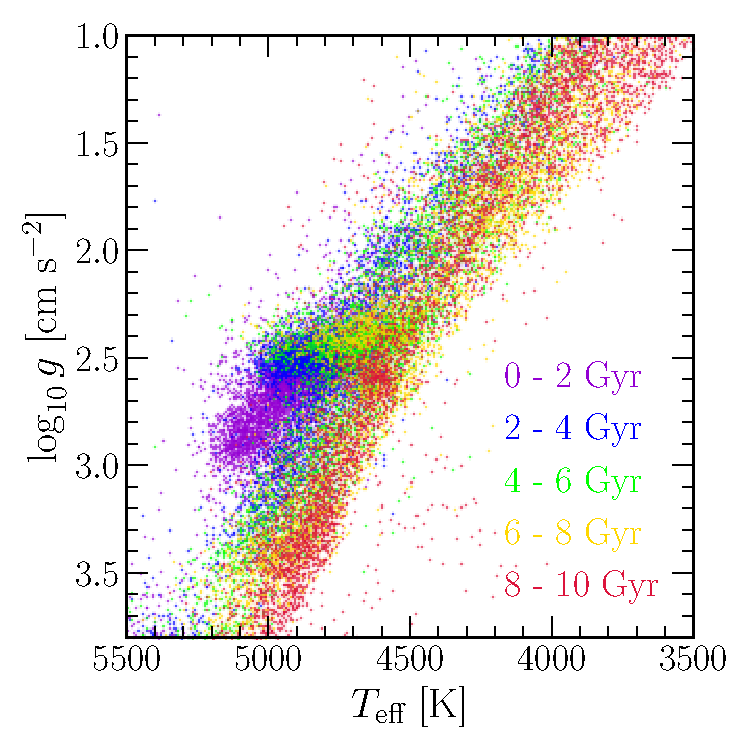
\includegraphics[scale = 0.6]{kiel_diagram.pdf}
\caption{
The Kiel diagram of our sample, color-coded by stellar age according to the
legend.
Within each age bin, we plot only a random subsample of~$N = 5000$ stars.
}
\label{outflows:fig:kiel-diagram}
\end{figure}

Fig.~\ref{outflows:fig:kiel-diagram} shows the Kiel diagram of a subsample of
our stars binned by age.
Comparing the distributions of stars along the red giant branch and red clump
between age bins indicates some systematic biases present in the sample.
The youngest stars are preferentially located in the red clump, whereas the
oldest stars distribute themselves much more evenly along the red giant branch.
This result is unsurprising as systematic uncertainties in APOGEE tend to
present as spurious correlations with~$T_\text{eff}$ and~$\log g$
\citep[e.g.,][]{Joensson2018, Eilers2022}.
However, we do not expect these systematic effects to impact our
characterizations of radial age and metallicity gradients (see discussion
in~\S~\ref{outflows:sec:results:caveats} below).

% Although there is no analytic expression for the peak, given the mean~$\mu$ and
% standard deviation~$\sigma$ of the corresponding unskewed distribution, an
% accurate numerical approximation is given by~$\mu + m_0 \sigma$, where
% \begin{equation}
% m_0 \equiv \sqrt{\frac{2}{\pi}}
% \left[
% \delta - \left(\frac{4 - \pi}{2}\right)
% \frac{\delta^3}{\pi - 2\delta^2}
% \right] - \frac{\text{sign}(a)}{2} e^{-2\pi / \left|a\right|}
% \end{equation}
% for~$\delta \equiv a / \sqrt{1 + a^2}$ defined in terms of the skewness
% parameter~$a$~\citep{Azzalini2014}.





